\clearpage
\begin{usecaseinstance}
  \addheading{Use-Case Instance}
  \adddoublerow{Name}{Simple and Complete DeployAndRun Instance} 
  \adddoublerow{Instance ID}{01}
  \adddoublerow{Environmental conditions and assumptions}{The necessary IT infrastructure exists to allow for deployment of the \msricrash system.}
  \adddoublerow{Inputs}{inputs are sequences of characters interpreted as string or numbers.}
  
\addrowheading{Instance flow description}
\addnumberedsinglerow{}{the \msrcode{actMsrCreator} actor \msrcode{theCreator}
sends the message \msrcode{oeCreateSystemAndEnvironment(1)} requesting the
initialization of the system and its environment (consisting of one
administrator identified here by \msrcode{bill}) and indicating that the number of communication company actor instances for the system's environment is 1 (identified here by \msrcode{tango}).
}
\addnumberedsinglerow{}{the \msrcode{actAdministrator} actor \msrcode{bill} sends the message \msrcode{oeLogin(icrashadmin,7WXC1359)} to securely connect to the system.}
\addnumberedsinglerow{}{the \msrcode{actAdministrator} actor \msrcode{bill}
sends the message
\msrcode{oeAddUser(1,Steve, pwdMessirExcalibur2017,1635242A75, 'Vehicular,
Pedestrian, Wildlife, Property, Injury',Coordinator)} to set up a coordinator
(i.e. identified here by \msrcode{steve}) and indicating his identification
information, ID (i.e. \msrcode{1}) and a password (i.e.
\msrcode{pwdMessirExcalibur2017}), id from a token(i.e.\msrcode{1635242A75}),
specifying his domain of expertise(i.e. \msrcode{'Vehicular, Pedestrian,
Wildlife, Property, Injury'}) and finally he designates the user as a
Coordinator(i.e.\msrcode{Cooridnator}).}
\addnumberedsinglerow{}{the \msrcode{actAdministrator} actor \msrcode{bill}
sends the message
\msrcode{oeAddUser(2, franklin, pwdMessirExcalibur, 1456872B82, Null,
DomainExpert)} create a domain expert who is one person(i.e. identified here by
\msrcode{franklin}) and indicating his user identification his identification,
ID(i.e.\msrcode{2}), password(i.e.\msrcode{pwdMessirExcalibur123}), id from a
token(i.e.\msrcode{14566872B82}), specifying the users domain of expertise
as(\msrcode{Null} meaning that the user has no specific domain and can
therefore only be an EMS user or Domain expert) and finally he designates the user as a
domain expert(i.e.\msrcode{DomainExpert}).}
\addnumberedsinglerow{}{the \msrcode{actAdministrator} actor \msrcode{bill}
sends the message
\msrcode{oeAddUser(3, barry, pwdEMSExcalibur321, 2436787C82, Null, EMS)} to set
up a EMS user who is any user in the EMS headquarters(i.e. identified here by
\msrcode{barry}) and indicating his user identification as ID(i.e.\msrcode{3}),
password (i.e.\msrcode{pwdEMSExcalibur421}), id from a
token(i.e.\msrcode{2436787C82}), specifying the users domain of expertise
as(i.e.\msrcode{Null} meaning that the user has no specific domain and can
therefore only be an EMS user or DomainExpert) and finally he designates the
user as an EMS user(i.e.\msrcode{EMS}).}
\addnumberedsinglerow{}{the \msrcode{actAdministrator} actor \msrcode{bill} sends the message \msrcode{oeLogout()} to disconnect from the system.}
\addnumberedsinglerow{}{the \msrcode{actComCompany} actor \msrcode{tango} sends
the message \msrcode{oeAlert(witness, 2017-11-26-at-10-10-16AM,+3524666445252, 49.627675-6.159590, '3 cars involved in an accident.')} to transfer a declaration of a car crash by a witness indicating specific phone number, the date and time, the GPS coordinates of the witnessed car crash and a short message giving additional details.}
\addnumberedsinglerow{}{the \msrcode{actDomainExpert}actor \msrcode{franklin}
sends the message \msrcode{oeLogin(franklin, pwdMessirExcalibur123,
687594FAD9)}to securely connect to the system entering his
login(i.e.\msrcode{franklin}), his
password(i.e.\msrcode{pwdMessirExcalibur123})and entering his serial key that
he reads form a token device given to him by the administrator(i.e.687594FAD9).}
\addnumberedsinglerow{}{the \msrcode{actEMS}actor \msrcode{barry}
sends the message \msrcode{oeLogin(barry, pwdEMSExcalibur321,
24367872C282)}to securely connect to the system entering his
login(i.e.\msrcode{barry}), his
password(i.e.\msrcode{pwdEMSExcalibur321})and entering his serial key that
he reads form a token device given to him by the
administrator(i.e.\msrcode{24367872C282)}.}
\addnumberedsinglerow{}{the \msrcode{actDomainExpert} actor \msrcode{franklin}
sends the message
\msrcode{oeValidateAlert(1,49.627675-6.159590,2017-11-26-at-10-10-16AM,
valid, 'Vehicular, Pedestrian')}to validate the crisis and to set a Domain to
it.}
\addnumberedsinglerow{}{the \msrcode{actDomainExpert} actor \msrcode{franklin}
sends the message \msrcode{oeSollicitateCrisisHandling()} indicating that there
is a declared alert that is still not handled by any coordinator.}
\addnumberedsinglerow{}{the \msrcode{actCoordinator} actor \msrcode{steve} sends
the message \msrcode{oeLogin(steve, pwdMessirExcalibur2017, 63524275D9)} to
securely connect to the system, entering his login(i.e.\msrcode{steve}), his
password(i.e.\msrcode{pwdMessirExcalibur2017 }) and his serial Key that he reads form a token device he is given by the administrator(i.e.\msrcode{63524275D9})} 
\addnumberedsinglerow{}{the \msrcode{actCoordinator} actor \msrcode{steve} sends
the message \msrcode{oeGetAlertsSet(valid)} to receive information about all the
pending crisis.} \addnumberedsinglerow{}{the \msrcode{actCoordinator} actor \msrcode{steve} sends the message \msrcode{oeSetCrisisHandler(1,Medium, in-handling, 49.627095-6.160251, 2017-11-26-at-10-10-16AM)} to declare that he is taking care of the alert with the ID equal to \msrcode{1} which becomes the Crisis Id, sets the crisis type to(i.e.\msrcode{Medium}, the crisis type to(i.e.\msrcode{in-handling}), enters the GPS coordinates and the date and time.}
\addnumberedsinglerow{}{the \msrcode{actComCompany} actor \msrcode{tango} sends the message \msrcode{oeAlert(witness, 2017-11-26-at-10-20-18AM,+3524666445314, 49.627095-6.160251,�Please send rescue services.�)} to
transfer a declaration of a car crash by a witness indicating specific the phone number, the date and
time, the GPS coordinates of the witnessed car crash and a short message giving additional details. 
This alert's GPS coordinates match the previous alert sent coordinates in step
7 and the time elapsed between the two alerts is 10 minutes therefore the alert
is considered to be originating from the same location.
}
\addnumberedsinglerow{}{the \msrcode{actDomainExpert} actor \msrcode{franklin}
sends the message \msrcode{oeValidateAlert(1,49.627675-6.159590,2017-11-26-at-10-10-16AM, valid, 'Vehicular, Pedestrian')}to validate the crisis and to set a Domain to it. Because the alert originated from the same location and only 10 min later it an automated message informs the Domain Expert to validate it to the same alert ID as the previous alert.}
\addnumberedsinglerow{}{the \msrcode{actCoordinator} actor steve send the
message \msrcode{oeReportOnCrisis(1, ' 2 Alerts received about a car accident at the same location apparently involving 3 vehicles', 2, Medium, Handled,'witness, 2017-11-26-at-10-10-16AM,+3524666445252,
49.627675-6.159590,'3 cars involved in an accident', witness, 2017-11-26-at-10-2-18AM,+3524666445314, 49.627095-6.160251,'Please send rescue services.',3, 3)}
indicating the crisis ID(i.e.1), entering a specific comment in the comment area(i.e.\msrcode{'2Alertsrecived about a car accident at the same location apparently involving 3 vehicles'}),
specifying his user ID(i.e.\msrcode{2}), setting the CrisisType(i.e.\msrcode{Medium}), indicating the current crisisStatus(\msrcode{handled}), entering the previous received alerts,
indicating the number of vehicles involved in the accident(i.e.\msrcode{3}) and entering the number of victims(i.e.\msrcode{3}) because he suspects that there may be 3 victims due to the amount of cars involved in the accident.
Entering a preliminary report on the crisis with the information that he presumes are right.}
\addnumberedsinglerow{}{the \msrcode{actCoordinator} actor \msrcode {steve} send
the message \msrcode{oeRequestEMSAssistance('We have received an Alert of an accident involving 3 cars from 1 victim and 1 witness at the same location please send police and ambulance',1, 49.627095-6.160251, 3,3, Ambulance Police)}, entering a comment(i.e. \msrcode{' We have received an Alert of an accident involving 3 cars from 1 victim and 1 witness at the same location please send Police assistance'}), indicating the RequestID(i.e.\msrcode{1}), entering the GPS location of the accident(i.e.\msrcode{49.627095-6.160251}), informing them of the number of cars involved(i.e.\msrcode{3}) and informing them of the presumed number of victims(i.e.\msrcode{3}) requesting emergency services assistance(i.e.\msrcode{Ambulance, Police}).}
\addnumberedsinglerow{}{the \msrcode{actCooordinator} actor steve sends the message \msrcode{oeSetCrisisStatus(1, handled)}to change the status of the crisis identified by the ID(i.e.\msrcode{1}) to the status(i.e.\msrcode{handled}) thus indicating that he has handled the situation for now but it's not solved yet.}
\addnumberedsinglerow{}{the \msrcode{actEMS} actor \msrcode{barry} sends the
message \msrcode{oeReplyToRequest(1,'Message received, dispatching police and ambulance units.', 1, Handled)} indicating the CrisisID(i.e.\msrcode{1}), sending the comment(i.e.\msrcode{'Message received, dispatching police and ambulance units.'}), to confirm that the request with the ID(i.e.\msrcode{1}) has been received and is being handled, indicated by the EMS crisis status(i.e. \msrcode{Handled}).}
\addnumberedsinglerow{}{the \msrcode{actEMS} actor \msrcode{barry} sends the
message \msrcode{oeReportEMSCrisisStatus(1, 'Units arrived on scene report 4 victims, 3 cars involved in accident. Situation under control 1 victim brought Mercy hospital', solved, Mercy Hospital, Jeremy Springer, John Snow, +32168432)} indicating the crisis ID(i.e.\msrcode{1}), adding a comment(i.e. \msrcode{'Units arrived on scene report 4 victims, 3 cars involved in accident. Situation under control 1 brought to Mercy hospital'}), specifying the EMS crisis status as solved (i.e.\msrcode{solved}), indicating the hospital name as (i.e.\msrcode{Mercy Hospital}), indicating the victim name(i.e.\msrcode{Jeremy Springer}), indicating the victims ICE contact's name as(i.e.\msrcode{John Snow}) and the contacts phone number as (\msrcode{+32168432})  to report on the EMS crisis Status.}
\addnumberedsinglerow{}{the \msrcode{actComCompany} actor \msrcode{tango} sends
message \msrcode{oeInfoFam('Dear John Snow, I regret to inform you that Jeremy Springer was in a car accident involving 3 other cars. Jeremy Springer was brought to the Mercy hospital for examination. Regretfully yours..',Jeremy Springer, +32168432, Mercy Hospital)} to inform the victims family members about the state of the victim and in which hospital they reside.}
\addnumberedsinglerow{}{the \msrcode{actCoordinator} actor \msrcode{steve} sends
the message \msrcode{oeReportOnCrisis(1, ' 2 Alerts received about a car accident at the same location involving 3 vehicles and 4 victims one victim Jeremy Springer was brought to the Mercy hospital.', 2, Medium, Handled,'witness, 2017-11-26-at-10-10-16AM,+3524666445252, 49.627675-6.159590,'3 cars involved in an accident 'witness, 2017-11-26-at-10-2-18AM,+3524666445314, 49.627095-6.160251,'Please send rescue services.'',3, 4)} to set the report for the crisis with ID equal to 1 that he is handling.}
\addnumberedsinglerow{}{the \msrcode{actCoordinator} actor \msrcode{steve} sends the message \msrcode{oeReportOnCrisis(1,'3 victims sent to hospital, 2 cars evacuated and 4 rescue unit mobilized')} to set the report for the crisis with \msrcode{ID} equal to 1 that he is handling.}
\addnumberedsinglerow{}{the \msrcode{actCoordinator} actor \msrcode{steve} sends the message \msrcode{oeCloseCrisis(1)} to declare the crisis with ID equal to \msrcode{1} as closed.
}
  \adddoublerow{Outputs}{at the end of this instance flow the system should have its environment made of one communication company actor instance, one coordinator actor instance, one administrator instance and the creator instance. The system state should contain two alerts defined according to the information received from the communication company, only one crisis that should be considered as solved and being alerted by the two alerts received.}
\end{usecaseinstance}  

 \begin{figure}[htbp]
 \begin{center} 
 \scalebox{0.95}{
 %\includegraphics{image} 
 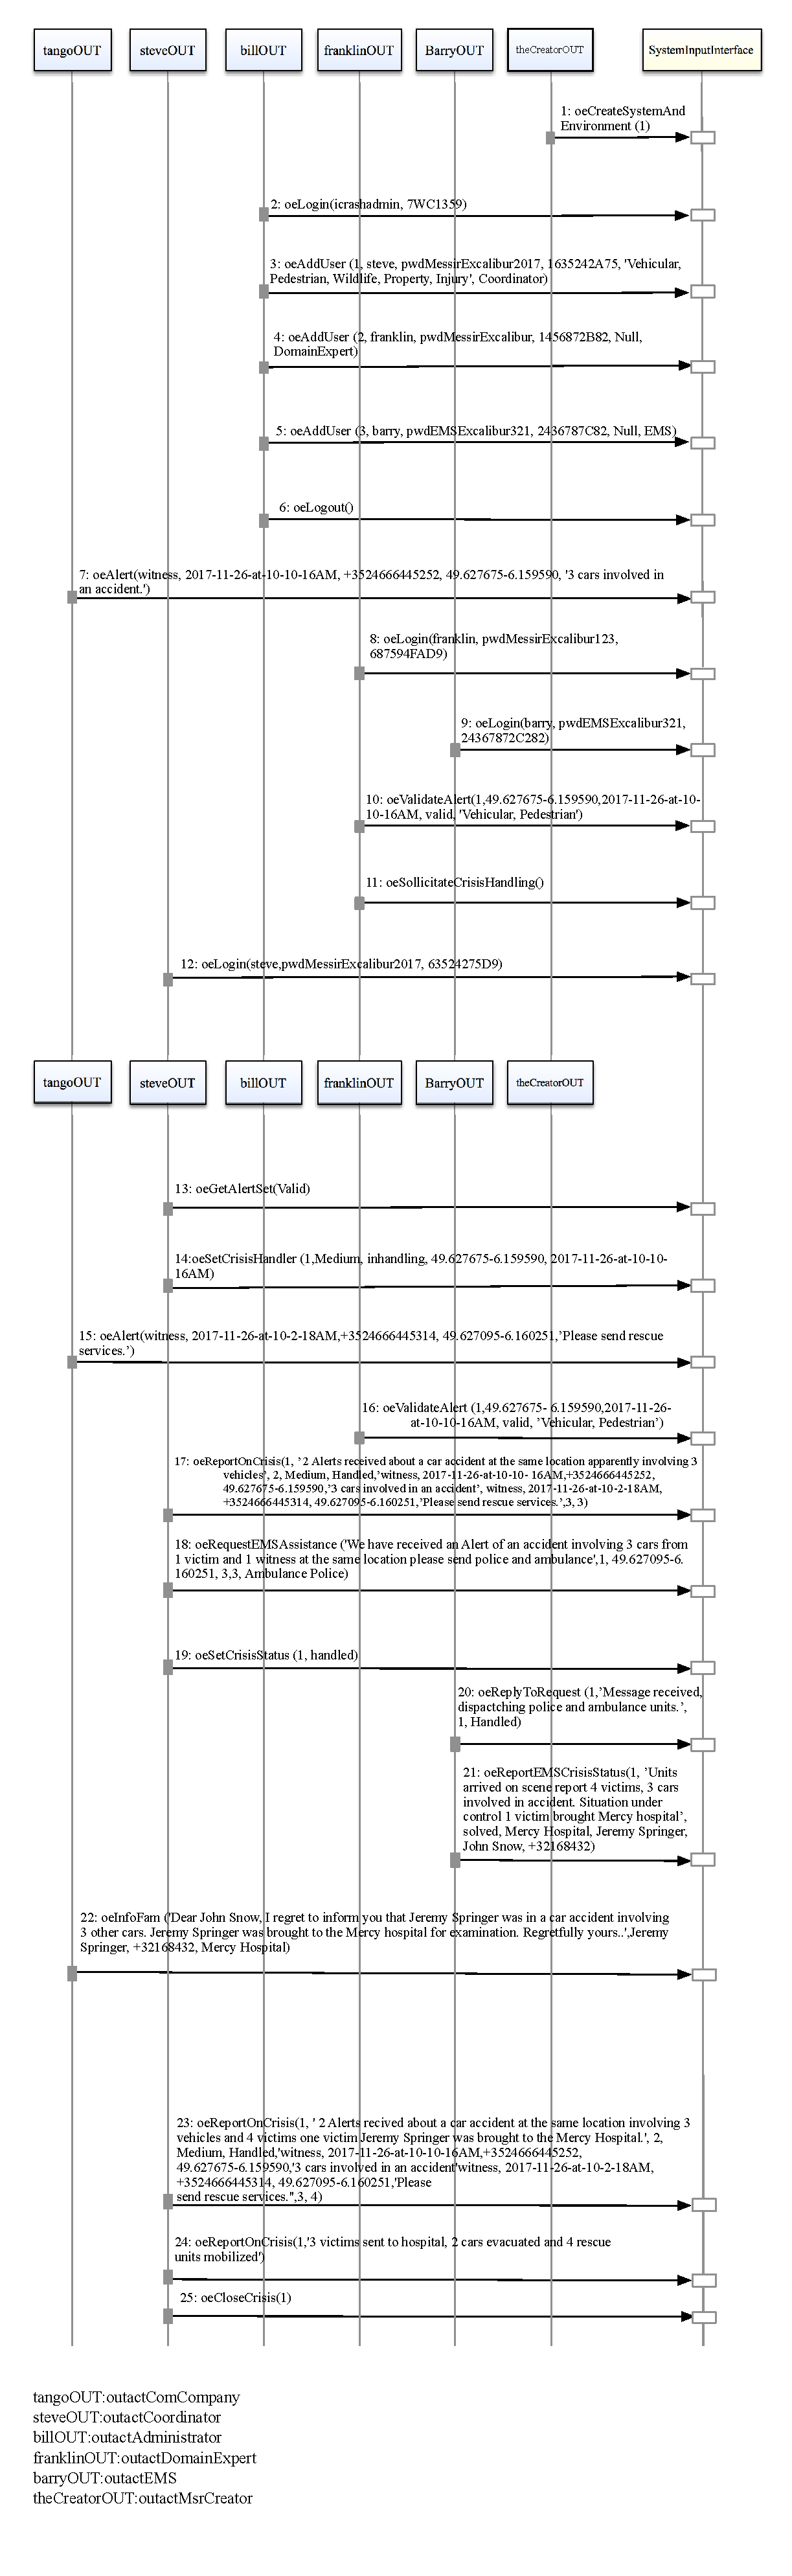
\includegraphics[width=180mm]{./images/SequenceDiagram.eps}
 \normalsize}
 \end{center}
 \caption[\msricrash Use Case Diagram:  SequenceDiagram Diagram]{\msricrash Use Case Diagram:  SequenceDiagram}
 \label{fig:icrash-RE-UCD- SequenceDiagram}
 \end{figure}
 \vspace{0.5cm}

